\documentclass[../../../../main.tex]{subfiles}

\begin{document}

\section*{1998年 東京大学 理科}

\noindent
東大の本気。ムズすぎワロタ\dots{} 1, 答えが予想できる3, ただのけいさんゲーの4, 6をといておけば後はもう時間との勝負だが\dots

\newpage

\subsection*{第1問}

\noindent
\textbf{[解]} $t = a - \frac{1}{a}$ とおく. $f(x) = (3x^2 - 4)(x - t)$ より, $f'(x) = 9x^2 - 6tx - 4$ で, $f'(0) = -4 < 0$ 及び 2次係数正から, $f'(x) = 0$ は 2解 $\alpha, \beta$ ($\alpha < \beta$) を持つ. $x = \alpha$ で極大となることから,
\begin{align*}
(\text{極大}) - (\text{極小}) &= f(\alpha) - f(\beta) = \int_{\beta}^{\alpha} f'(x) \, dx = -\int_{\alpha}^{\beta} 9(x - \alpha)(x - \beta) \, dx \\
&= \frac{3}{2}(\beta - \alpha)^3
\end{align*}
となる. したがって, $\beta - \alpha > 0$ とあわせて, $\beta - \alpha$ が $\min$ となるような $a$ をもとめれば良い.

$\alpha < \beta$ から
\[
\beta - \alpha = 2 \frac{\sqrt{9t^2 + 36}}{9} = \frac{2}{3} \sqrt{t^2 + 4}
\]
したがって, $t^2$ が最小の時, $\beta - \alpha$ は最小. 右図から, もとめるのは $t = 0$ となる $a = \pm 1$.

\begin{center}
\begin{tikzpicture}[scale=0.8, >=stealth]
\draw[->] (-3,0) -- (3,0) node[right] {$a$};
\draw[->] (0,-3) -- (0,3) node[above] {$t$};
\node[below left] at (0,0) {$O$};
\draw[domain=0.35:2.8, smooth, variable=\x, thick] plot ({\x}, {\x - 1/\x});
\draw[domain=-2.8:-0.35, smooth, variable=\x, thick] plot ({\x}, {\x - 1/\x});
\draw[dashed] (-2.5,-2.5) -- (2.5,2.5) node[above right] {$t = a - \frac{1}{a}$};
\filldraw (1,0) circle (1.5pt) node[below right] {$1$};
\filldraw (-1,0) circle (1.5pt) node[above left] {$-1$};
\end{tikzpicture}
\end{center}

\newpage

\subsection*{第2問}

\noindent
\textbf{[解]} $z = k \in \mathbb{Z}$ と固定すると,
\[
\begin{cases}
x + y \le n - k \\
-x + y \le n + k \\
x - y \le n + k \\
-x - y \le n - k
\end{cases}
\iff
\begin{cases} -(n-k) \le x + y \le n - k \\ -(n+k) \le x - y \le n + k \end{cases} \quad \dots \text{①}
\]
これをみたす $(x, y)$ の存在条件から, $-n \le k \le n \ \dots \text{②}$ である. このもとで①を図示すると右図斜線部(境界含む). この内部にある格子点の数を $S(k)$ とおく. ここで 1辺 $2n$ の正方形から, 三角形4つを取り去ることで $S(k)$ をもとめる. まず, 右図1のような正方形の周及び内部の格子点は
\[
(2n + 1)^2 \quad \dots \text{③}
\]
である. 対称性から, 以下 $k \ge 0$ とする. 右の図のように各点を定める. ここで, $\triangle ABH, \triangle BCD, \triangle DEF, \triangle FGH$ は, 各々1辺が $n-k, n+k, n-k, n+k$ の直角2等辺三角形である. $\dots \text{④}$

ここで, 1辺 $p \in \mathbb{N}$ の直角2等辺三角形の周及び内部(斜辺をのぞく)の格子点は, 右図2から,
\[
1 + 2 + \dots + p = \frac{1}{2} p (p + 1) \quad \dots \text{⑤}
\]
である. よって, ④⑤から, $\triangle ABH, \triangle BCD, \triangle DEF, \triangle FGH$ の周及び内部(斜辺除く)にある格子点はあわせて
\[
(n+k)(n+k+1) + (n-k)(n+1-k) \quad \dots \text{⑥}
\]
である. ③⑥から,
\[
S(k) = (2n+1)^2 - (n+k)(n+1+k) - (n-k)(n+1-k) \quad \dots \text{⑦}
\]
である. したがって対称性から, もとめる格子点の数は, ②とあわせて,
\[
f(n) = S(0) + 2 \sum_{k=1}^n S(k) \quad \dots \text{⑧}
\]
である. ⑦から
\[
\begin{cases}
S(0) = 2n^2 + 2n + 1 \\
\displaystyle\sum_{k=1}^n S(k) = n(2n+1)^2 - \sum_{k=1}^n (k+n)(k+1+n) - \sum_{k=1}^n (n-k)(n-1-k)
\end{cases} \quad \dots \text{⑨}
\]
であり,
\begin{align*}
\sum_{k=1}^n (k+n)(k+1+n) &= \frac{1}{3} \sum_{k=1}^n \left\{ (k+n)(k+1+n)(k+n+2) - (k+n-1)(k+n)(k+n+1) \right\} \\
&= \frac{1}{3} \left\{ (2n)(2n+1)(2n+2) - n(n+1)(n+2) \right\} = \frac{n(n+1)}{3} (7n + 2) \\
\sum_{k=1}^n (k-n)(k-n-1) &= \frac{1}{3} \sum_{k=1}^n \left\{ (k+1-n)(k-n)(k-1-n) - (k-n)(k-1-n)(k-2-n) \right\} \\
&= \frac{1}{3} \left\{ -(-1)(-n)(-1-n) \right\} = \frac{1}{3} n(n+1)(n-1)
\end{align*}
を⑨に代入して,
\[
\sum_{k=1}^n S(k) = (2n+1)^2 \cdot n - \frac{1}{3} n(n+1)(7n+2) - \frac{1}{3} n(n+1)(n-1)
\]
だから, ⑧とあわせて
\begin{align*}
\frac{f(n)}{n^3} &= \frac{S(0)}{n^3} + 2 \left[ \left(2 + \frac{1}{n}\right)^2 - \frac{1}{3}\left(1 + \frac{1}{n}\right)\left(7 + \frac{2}{n}\right) - \frac{1}{3}\left(1 + \frac{1}{n}\right)\left(1 - \frac{1}{n}\right) \right] \\
&\xrightarrow{n \to \infty} 0 + 2 \left[ 4 - \frac{7}{3} - \frac{1}{3} \right] = \frac{8}{3} \quad \left( \because \frac{S(0)}{n^3} \to 0 \right)
\end{align*}

\begin{center}
\begin{tikzpicture}[scale=0.7, >=stealth]
\draw[->] (-4,0) -- (4,0) node[right] {$x$};
\draw[->] (0,-4) -- (0,4) node[above] {$y$};
\fill[gray!20] (-3,1) -- (-1,3) -- (3,1) -- (3,-1) -- (1,-3) -- (-3,-1) -- cycle;
\draw[thick] (-3,1) -- (-1,3) -- (3,1) -- (3,-1) -- (1,-3) -- (-3,-1) -- cycle;
\draw[dashed] (-3,-3) rectangle (3,3);
\node[above left] at (-3,1) {$A$};
\node[above] at (-1,3) {$B$};
\node[above right] at (3,3) {$C$};
\node[right] at (3,1) {$D$};
\node[below right] at (3,-3) {$E$};
\node[below] at (1,-3) {$F$};
\node[below left] at (-3,-3) {$G$};
\node[left] at (-3,-1) {$H$};
\node[below] at (-3,0) {$-n$};
\node[below] at (3,0) {$n$};
\node[left] at (0,3) {$n$};
\node[left] at (0,-3) {$-n$};
\node[above] at (0,3.3) {(図1)};
\end{tikzpicture}
\qquad
\begin{tikzpicture}[scale=0.7, >=stealth]
\draw[->] (-0.5,0) -- (4,0) node[right] {$x$};
\draw[->] (0,-0.5) -- (0,4) node[above] {$y$};
\draw[thick] (0,3) -- (3,0) node[midway, above right] {$x+y=p$};
\draw[dashed] (0,3) -- (0,0) -- (3,0);
\filldraw (0,3) circle (2pt) node[left] {$p$};
\filldraw (3,0) circle (2pt) node[below] {$p$};
\node[below left] at (0,0) {$0$};
\node[above] at (1.5,3.3) {(図2)};
\end{tikzpicture}
\end{center}

\newpage

\subsection*{第3問}

\noindent
\textbf{[解]}

\begin{center}
\begin{tikzpicture}[scale=0.8, >=stealth]
\draw[->] (-0.5,0) -- (4.5,0) node[right] {$x$};
\draw (0.8, 0.8) circle (0.8);
\draw (2.5, 1.2) circle (1.2);
\draw (1.55, 0.25) circle (0.25);
\node at (0.8, 0.8) {$C_{n+1}$};
\node at (2.5, 1.2) {$C_n$};
\node at (1.55, 0.45) {$C_{n+2}$};
\filldraw (0.8,0) circle (1pt) node[below] {$x_{n+1}$};
\filldraw (2.5,0) circle (1pt) node[below] {$x_n$};
\filldraw (1.55,0) circle (1pt) node[below] {$x_{n+2}$};
\node[above] at (2, 2.5) {$n$ : odd の時};
\end{tikzpicture}
\qquad
\begin{tikzpicture}[scale=0.8, >=stealth]
\draw[->] (-0.5,0) -- (4.5,0) node[right] {$x$};
\draw (0.8, 1.2) circle (1.2);
\draw (2.5, 0.8) circle (0.8);
\draw (1.75, 0.25) circle (0.25);
\node at (0.8, 1.2) {$C_n$};
\node at (2.5, 0.8) {$C_{n+1}$};
\node at (1.75, 0.45) {$C_{n+2}$};
\filldraw (0.8,0) circle (1pt) node[below] {$x_n$};
\filldraw (2.5,0) circle (1pt) node[below] {$x_{n+1}$};
\filldraw (1.75,0) circle (1pt) node[below] {$x_{n+2}$};
\node[above] at (2, 2.5) {$n$ : even の時};
\end{tikzpicture}
\end{center}

円 $C_n$ の中心 $O_n$ とする. $O_{n+2}$ から $x = x_n, x_{n+1}$ への垂足を各 $H_n, H_{n+1}$ とおく.
$\triangle O_n H_n O_{n+2}, \triangle O_{n+1} H_{n+1} O_{n+2}$ に三平方を用いて,
\[
\begin{cases}
(r_{n+2} + r_n)^2 = (x_n - x_{n+2})^2 + (r_{n+2} - r_n)^2 \\
(r_{n+2} + r_{n+1})^2 = (x_{n+1} - x_{n+2})^2 + (r_{n+2} - r_{n+1})^2
\end{cases}
\]
\[
\begin{cases}
2\sqrt{r_n r_{n+2}} = |x_n - x_{n+2}| \\
2\sqrt{r_{n+1} r_{n+2}} = |x_{n+2} - x_{n+1}|
\end{cases}
\quad (\because r_k > 0)
\]
だから, $n$: even の時 $x_n < x_{n+2} < x_{n+1}$, $n$: odd の時 $x_{n+1} < x_{n+2} < x_n$ であることより,
\[
\begin{cases}
2\sqrt{r_n r_{n+2}} = (-1)^n (x_{n+2} - x_n) \\
2\sqrt{r_{n+1} r_{n+2}} = (-1)^n (x_{n+1} - x_{n+2})
\end{cases}
\quad \dots \text{①}
\]
又, $O_n, O_{n+1}$ に対しても同様に
\[
(r_{n+1} + r_n)^2 = (r_{n+1} - r_n)^2 + (x_{n+1} - x_n)^2
\]
\[
2\sqrt{r_n r_{n+1}} = (-1)^n (x_{n+1} - x_n) \quad \dots \text{②}
\]
が成立する.

\bigskip

(1) $q_n \in \mathbb{Z} \dots \spadesuit$ を帰納法で示す. $n=0, 1$ の時, $q_0 = q_1 = 1$ から $\spadesuit$ は成立するので, 以下 $n=k, k+1 \ (k \in \mathbb{Z}_{\ge 0})$ での成立を仮定する.
①で辺々足したものと②から
\[
2\sqrt{r_k r_{k+2}} + 2\sqrt{r_{k+1} r_{k+2}} = 2\sqrt{r_k r_{k+1}}
\]
$q_n = \frac{1}{2\sqrt{r_n}}$ から
\[
\frac{1}{q_k q_{k+2}} + \frac{1}{q_{k+1} q_{k+2}} = \frac{1}{q_k q_{k+1}}
\]
両辺に $q_k q_{k+1} q_{k+2}$ をかけて,
\[
q_{k+2} = q_k + q_{k+1} \in \mathbb{Z} \quad (\because \text{仮定}) \quad \dots \text{③}
\]
よって $n=k+2$ でも $\spadesuit$ は成立. 以上から $\spadesuit$ は示された. \hfill $\blacksquare$

\bigskip

(2) ①の辺々わって, $p_n = \frac{x_n}{2\sqrt{r_n}}$ から
\[
\begin{cases}
(-1)^n = (q_n p_{n+2} - q_{n+2} p_n) & \dots \text{④} \\
(-1)^n = (q_{n+2} p_{n+1} - q_{n+1} p_{n+2}) & \dots \text{⑤}
\end{cases}
\]
④, ⑤を代入して引いて,
\[
q_n(p_{n+1} + p_n) + q_{n+1}(p_n + p_{n+1}) = p_{n+2}(q_n + q_{n+1})
\]
$q_n + q_{n+1} \neq 0$ だから ($\because q_n > 0$),
\[
p_n + p_{n+1} = p_{n+2} \quad \dots \text{⑥}
\]
が成り立つ. 以下, $p_n \in \mathbb{Z}$ かつ $p_n$ と $q_n$ が互いに素 $\dots \clubsuit$ であることを帰納的に示す.
$n=0, 1$ の時, $p_0 = 0, p_1 = 1$ となって $\clubsuit$ は成立するので, 以下 $n=k, k+1 \ (k \in \mathbb{Z}_{\ge 0})$ での成立を仮定する.
すると⑥から, $p_{k+2} \in \mathbb{Z}$ となる $\dots \text{⑦}$. さらに, 初期条件及び③, ⑥から,
$p_{n+1} = q_n$ となるので, 「$p_{k+2}$ と $q_{k+2}$ が互いに素」$\iff$「$q_{k+1}$ と $p_{k+2}$ が互いに素」$\iff$「$q_{k+1}$ と $q_{k+1} + q_k$ が互いに素」$(\because \text{③}) \iff$「$q_{k+1}$ と $q_k$ が互いに素」$\iff$「$q_{k+1}$ と $p_{k+1}$ が互いに素」となり, 仮定から $q_{k+2} \perp p_{k+2}$ となる $\dots \text{⑧}$
⑦, ⑧から $n=k+2$ でも $\clubsuit$ は成立. よって $\clubsuit$ は示された. \hfill $\blacksquare$

\bigskip

(3) (2)から, $p_{n+1} = q_n \ (n \ge 0)$. $p_0 = 0$ であるので,
\[
x_n = \begin{cases} 0 & (n = 0) \\ \dfrac{q_{n-1}}{q_n} & (n \ge 1) \end{cases}
\]
となる. ③の両辺 $q_k$ でわって,
\[
\frac{1}{x_{n+2}} = x_{n+1} + 1 \quad (n \ge 0)
\]
これより, $x_{n+1} = \dfrac{1}{1 + x_n} \quad (n \ge 1)$.
両辺 $\alpha = \dfrac{1}{1 + \alpha}$ を引いて,
\[
x_{n+1} - \alpha = \frac{1}{1 + x_n} - \frac{1}{1 + \alpha} = \frac{-1}{(1 + \alpha)(1 + x_n)} (x_n - \alpha)
\]
両辺絶対値をとって,
\[
|x_{n+1} - \alpha| = \left| \frac{1}{(1 + \alpha)(1 + x_n)} \right| |x_n - \alpha|
\]
ここで, $\alpha = \dfrac{-1 + \sqrt{5}}{2}$, $0 \le x_n \le 1$ から
\[
|x_{n+1} - \alpha| \le \left| \frac{\sqrt{5}-1}{2} \right| |x_n - \alpha| < \frac{2}{3} |x_n - \alpha|
\]
なので, くり返し用いて,
\[
|x_n - \alpha| < \left(\frac{2}{3}\right)^{n-2} |x_2 - \alpha|
\]
はさみうちから, $x_n \longrightarrow \alpha = \dfrac{-1 + \sqrt{5}}{2}$ である.

\newpage

\subsection*{第4問}

\noindent
\textbf{[解1]} $f(x) = \dfrac{x^2(2 \cdot 3^3 \cdot n - x)}{2^5 \cdot 3^2 \cdot n^2}$ において, $k \in \mathbb{Z}$ として,
\[
\begin{cases}
|f(k+1) - f(k)| \le 1 \text{ なら, } [f(k+1)] = [f(k)], [f(k)] \pm 1 \\
|f(k+1) - f(k)| \ge 1 \text{ なら, } [f(k+1)] \neq [f(k)]
\end{cases}
\quad \dots \text{＊}
\]
である.
\begin{align*}
f(k+1) - f(k) &= \frac{1}{2^5 \cdot 3^2 \cdot n^2} \left[ (k+1)^2(2 \cdot 3^3 \cdot n - k - 1) - k^2(2 \cdot 3^3 \cdot n - k) \right] \\
&= \frac{1}{2^5 \cdot 3^2 \cdot n^2} \left[ (2k+1)(2 \cdot 3^3 \cdot n - k) - (k+1)^2 \right] \\
&= \frac{1}{2^5 \cdot 3^2 \cdot n^2} \left[ -3k^2 + (2 \cdot 3^3 \cdot n - 3)k + 2 \cdot 3^3 \cdot n - 1 \right] \quad \dots \text{①}
\end{align*}
ここで, $2^5 \cdot 3^2 \cdot n^2 \cdot f'(x) = 3x(2^2 \cdot 3^2 \cdot n - x)$ から, $0 \le x \le 36n$ では $f'(x) \ge 0$ となり, $f(x)$ は単調増加である. $g(k) = f(k+1) - f(k) - 1$ とおくと, ①から,
\[
2^5 \cdot 3^2 \cdot n^2 g(k) = -3k^2 + 3(2^2 \cdot 3^2 \cdot n - 1)k + 2 \cdot 3^3 \cdot n - 1 - 2^5 \cdot 3^2 \cdot n^2
\]
なので, $g(k) = 0$ の解は,
\begin{align*}
k &= \frac{1}{6} \left[ 3(2^2 \cdot 3^2 \cdot n - 1) \pm \sqrt{9(2^2 \cdot 3^2 \cdot n - 1)^2 - 12\left(2^5 \cdot 3^2 \cdot n^2 + 1 - 2 \cdot 3^3 \cdot n\right)} \right] \\
&= \frac{1}{6} \left[ 3(2^2 \cdot 3^2 \cdot n - 1) \pm \sqrt{2^4 \cdot 3^4 \cdot n^2 - 3} \right] \quad \dots \text{②}
\end{align*}
ここで $2^2 \cdot 3^2 \cdot n - 3 < \sqrt{2^4 \cdot 3^4 \cdot n^2 - 3} < 2^2 \cdot 3^2 \cdot n$ だから, $0 \le k$ の範囲で $g(k) \ge 0$ となる $k \in \mathbb{Z}$ は, ②から,
\[
12n \le k \le 24n - 1 \quad \dots \text{③}
\]
である. $f(x)$ の単調性および ＊ から,
\[
\begin{cases}
k = 0, 1, \dots, 12n-1 \text{ の時, } [f(k+1)] = [f(k)], [f(k)] + 1 \\
k = 12n, \dots, 24n-1 \text{ の時, } [f(k+1)] > [f(k)] \\
k = 24n, \dots, 36n \text{ の時, } [f(k+1)] = [f(k)], [f(k)] + 1
\end{cases}
\]
だから,
\[
[f(0)] \le [f(1)] \le \dots \le [f(12n)] < [f(12n+1)] < \dots < [f(24n)] \le \dots \le [f(36n)]
\]
となり,
\[
[f(0)] = 0, \quad [f(12n)] = 7n, \quad [f(24n)] = 20n, \quad [f(36n)] = 27n
\]
だから求めるのは
\[
(7n + 1) + (24n - 1 - 12n) + (27n + 1 - 20n) = 26n + 1 \text{ 個}
\]

\begin{center}
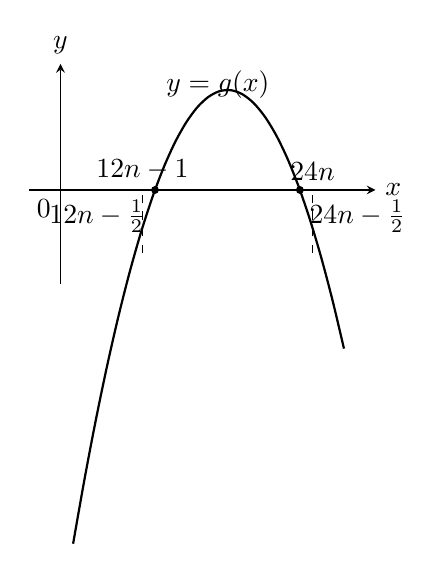
\begin{tikzpicture}[scale=0.8, >=stealth]
\draw[->] (-0.5,0) -- (5,0) node[right] {$x$};
\draw[->] (0,-1.5) -- (0,2) node[above] {$y$};
\draw[domain=0.2:4.5, smooth, variable=\x, thick] plot ({\x}, {-1.2*(\x-1.5)*(\x-3.8)});
\node[above] at (2.5, 1.3) {$y = g(x)$};
\filldraw (1.5,0) circle (1.5pt) node[below left] {$12n - \frac{1}{2}$};
\filldraw (3.8,0) circle (1.5pt) node[below right] {$24n - \frac{1}{2}$};
\draw[dashed] (1.3, -1) -- (1.3, 0) node[above] {$12n-1$};
\draw[dashed] (4.0, -1) -- (4.0, 0) node[above] {$24n$};
\node[below left] at (0,0) {$0$};
\end{tikzpicture}
\end{center}

\bigskip

\noindent
\textbf{[解2]} (以下) 平均値の定理から,
\[
f(k+1) - f(k) = f'(a_k) \quad (k < a_k < k+1) \quad \dots \text{①'}
\]
を満たす $a_k$ がある.
\[
f'(x) = \frac{x(2^2 \cdot 3^2 \cdot n - x)}{2^5 \cdot 3^2 \cdot n^2} \le 1 \iff -x^2 + 2^2 \cdot 3^2 \cdot n \cdot x - 2^5 \cdot 3^2 \cdot n^2 \le 0 \iff x \le 12n, 24n \le x
\]
だから, ①'とあわせて
\[
\begin{cases}
k = 0, 1, \dots, 12n-1 \text{ の時, } f(k+1) - f(k) < 1 \\
k = 12n, 12n+1, \dots, 24n-1 \text{ の時, } f(k+1) - f(k) > 1 \\
k = 24n, 24n+1, \dots, 36n \text{ の時, } f(k+1) - f(k) < 1
\end{cases}
\]
となって[解1]の③に帰着する.

\newpage

\subsection*{第5問}

\noindent
\textbf{[解]} $C = \cos\theta, S = \sin\theta$ とおく. $x_1 = 1, y_1 = 0$ である $\dots \text{①}$. $A_n = \vec{a} \cdot \vec{OP_n}$, $B_n = \vec{b} \cdot \vec{OP_n}$ とすると,
\[
\vec{OP_{n+1}} = 4(\vec{OP_n} - A_n \vec{a}) - 4(B_n - A_n \vec{a} \cdot \vec{b}) \vec{b} \quad \dots \text{②}
\]
であり,
\[
A_n = C x_n + S y_n, \quad B_n = \frac{1}{2}(\sqrt{3} x_n + y_n), \quad \vec{a} \cdot \vec{b} = \frac{1}{2}(\sqrt{3} C + S) \quad \dots \text{③}
\]
より, $T = \vec{a} \cdot \vec{b}$ とおいて, ②から
\begin{align*}
x_{n+1} &= (4 - 4C^2 - 3 + 2\sqrt{3}CT) x_n + (-4SC - \sqrt{3} + 2\sqrt{3}ST) y_n \\
&= (1 - C^2 + \sqrt{3}SC) x_n + (-SC - \sqrt{3}C^2) y_n \\
&= S(S + \sqrt{3}C) x_n - C(S + \sqrt{3}C) y_n \quad \dots \text{④} \\
y_{n+1} &= (-4CS - \sqrt{3} + 2CT) x_n + (4 - 4S^2 - 1 + 2ST) y_n \\
&= (-\sqrt{3}S^2 - 3CS) x_n + (3C^2 + \sqrt{3}CS) y_n \\
&= -\sqrt{3} S(S + \sqrt{3}C) x_n + \sqrt{3} C(S + \sqrt{3}C) y_n \quad \dots \text{⑤}
\end{align*}
ここで, $\alpha = S(S + \sqrt{3}C), \ \beta = C(S + \sqrt{3}C)$ とすると,
\[
\begin{cases}
x_{n+1} = \alpha x_n - \beta y_n \\
y_{n+1} = -\sqrt{3} (\alpha x_n - \beta y_n)
\end{cases}
\quad \dots \text{①'}
\]
だから, $y_{n+1} = -\sqrt{3} x_{n+1} \ (n \ge 1)$ なので,
\[
x_{n+1} = (\alpha + \sqrt{3}\beta) x_n \quad (n \ge 2)
\]
くり返し用いて,
\[
\begin{cases}
x_n = (\alpha + \sqrt{3}\beta)^{n-2} x_2 & (n \ge 2) \\
y_n = -\sqrt{3} (\alpha + \sqrt{3}\beta)^{n-2} x_2 & (n \ge 2)
\end{cases}
\quad \dots \text{⑦}
\]
ここで, ①'から $x_2 = \alpha x_1 = \alpha$ だから, ①'から
\[
\begin{cases}
x_n = \alpha (\alpha + \sqrt{3}\beta)^{n-2} \\
y_n = -\sqrt{3}\alpha (\alpha + \sqrt{3}\beta)^{n-2}
\end{cases}
\quad (n \ge 2) \quad \dots \text{⑦'}
\]
したがって, 数列 $\{x_n\}, \{y_n\}$ が収束する条件は,
\[
-1 < \alpha + \sqrt{3}\beta \le 1 \quad \text{or} \quad \alpha = 0
\]
である. $\alpha, \beta$ に値を代入して
\[
-1 < (S + \sqrt{3}C)^2 \le 1 \quad \text{or} \quad S = 0 \text{ or } S + \sqrt{3}C = 0
\]
\[
\iff -1 \le S + \sqrt{3}C \le 1 \quad \text{or} \quad S = 0 \quad \dots \text{⑧}
\]
ここで, $S + \sqrt{3}C = 2 \sin\left(\theta + \frac{\pi}{3}\right)$ だから, $-1 \le S + \sqrt{3}C \le 1 \iff -\frac{1}{2} \le \sin\left(\theta + \frac{\pi}{3}\right) \le \frac{1}{2}$ に注意して,
\[
⑧ \iff \frac{5}{6}\pi \le \theta + \frac{\pi}{3} \le \frac{7}{6}\pi, \ \frac{11}{6}\pi \le \theta + \frac{\pi}{3} \le \frac{13}{6}\pi \quad \text{or} \quad \theta = 0, \pi
\]
\[
\iff \frac{1}{2}\pi \le \theta \le \frac{5}{6}\pi \quad \text{or} \quad \frac{3}{2}\pi \le \theta \le \frac{11}{6}\pi \quad \text{or} \quad \theta = 0, \pi
\]
だから, ①'に注意して, $\sin\left(\theta + \frac{\pi}{3}\right) = \pm \frac{1}{2} \iff \theta = \frac{1}{2}\pi, \frac{5}{6}\pi, \frac{3}{2}\pi, \frac{11}{6}\pi$ より

$1^\circ$ $\frac{1}{2}\pi < \theta < \frac{5}{6}\pi, \ \frac{3}{2}\pi < \theta < \frac{11}{6}\pi, \ \theta = 0, \pi$ の時
$x_n, y_n$ 共に 0 に収束.

$2^\circ$ $\theta = \frac{1}{2}\pi, \frac{5}{6}\pi, \frac{3}{2}\pi, \frac{11}{6}\pi$ の時
$x_n \to \alpha, \ y_n \to -\sqrt{3}\alpha$ となるから, $\alpha = S(S + \sqrt{3}C)$ から,
$\theta = \frac{1}{2}\pi, \frac{3}{2}\pi$ の時, $x_n \to 1, \ y_n \to -\sqrt{3}$
$\theta = \frac{5}{6}\pi, \frac{11}{6}\pi$ の時, $x_n \to -\frac{1}{2}, \ y_n \to \frac{\sqrt{3}}{2}$
である.

以上まとめて,
\[
\begin{cases}
\theta = 0, \ \frac{1}{2}\pi < \theta < \frac{5}{6}\pi, \ \theta = \pi, \ \frac{3}{2}\pi < \theta < \frac{11}{6}\pi \text{ の時}, & (x_n, y_n) \longrightarrow (0, 0) \\
\theta = \frac{1}{2}\pi, \ \frac{3}{2}\pi & (x_n, y_n) \longrightarrow (1, -\sqrt{3}) \\
\theta = \frac{5}{6}\pi, \ \frac{11}{6}\pi & (x_n, y_n) \longrightarrow \left(-\frac{1}{2}, \frac{\sqrt{3}}{2}\right)
\end{cases}
\]

\begin{center}
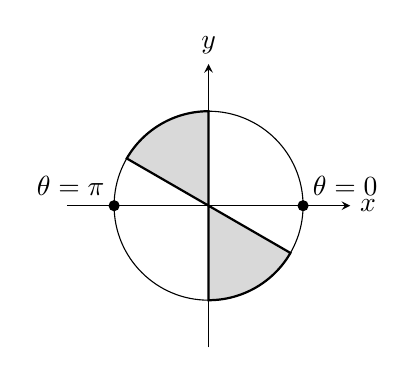
\begin{tikzpicture}[scale=1.2, >=stealth]
\draw[->] (-1.5,0) -- (1.5,0) node[right] {$x$};
\draw[->] (0,-1.5) -- (0,1.5) node[above] {$y$};
\draw (0,0) circle (1);
\draw[thick, fill=gray!30] (0,0) -- (90:1) arc (90:150:1) -- cycle;
\draw[thick, fill=gray!30] (0,0) -- (270:1) arc (270:330:1) -- cycle;
\filldraw (1,0) circle (1.5pt) node[above right] {$\theta=0$};
\filldraw (-1,0) circle (1.5pt) node[above left] {$\theta=\pi$};
\end{tikzpicture}
\end{center}

\newpage

\subsection*{第6問}

\noindent
\textbf{[解1]} 対称性から, $0 \le \theta \le \pi/4$ の部分での体積 $V'$ として, もとめる体積 $V$ は
\[
V = 8V' \quad \dots \text{①}
\]
である. $\theta$ を $0 \le \theta \le \pi/4$ とし, 以下 $C = \cos\theta, S = \sin\theta$ と表す. $x = C$ での切断面は右図斜線部
したがって, この平面での立体の面積 $S(\theta)$ として,
\[
S(\theta) = (C - S) \cdot 3(1-C)
\]
だから, もとめる体積は
\begin{align*}
V' &= \int_{\pi/4}^0 S(\theta) \, dc = \int_0^{\pi/4} S(\theta) \left( -\frac{dc}{d\theta} \right) d\theta \\
&= \int_0^{\pi/4} 3(1-C)(C-S) S \, d\theta \\
&= 3 \int_0^{\pi/4} (CS - S^2 - C^2 S + CS^2) \, d\theta \quad \dots \text{②}
\end{align*}
ここで,
\begin{align*}
\int_0^{\pi/4} SC \, d\theta &= \left[ -\frac{1}{4} \cos 2\theta \right]_0^{\pi/4} = \frac{1}{4} \\
\int_0^{\pi/4} S^2 \, d\theta &= \frac{1}{2} \left[ \theta - \frac{1}{2}\sin 2\theta \right]_0^{\pi/4} = \frac{1}{2}\left(\frac{\pi}{4} - \frac{1}{2}\right) \\
\int_0^{\pi/4} C^2 S \, d\theta &= \left[ -\frac{1}{3} C^3 \right]_0^{\pi/4} = \frac{1}{3} \left(1 - \frac{1}{2\sqrt{2}}\right) \\
\int_0^{\pi/4} S^2 C \, d\theta &= \left[ \frac{1}{3} S^3 \right]_0^{\pi/4} = \frac{1}{3} \frac{1}{2\sqrt{2}}
\end{align*}
から, ②に代入して
\[
V' = 3 \left[ \frac{1}{4} - \frac{1}{2}\left(\frac{\pi}{4} - \frac{1}{2}\right) - \frac{1}{3}\left(1 - \frac{1}{2\sqrt{2}}\right) + \frac{1}{3}\frac{1}{2\sqrt{2}} \right] = \frac{1}{2}(\sqrt{2} + 1) - \frac{3}{8}\pi
\]
①から
\[
V = 4(\sqrt{2}+1) - 3\pi
\]

\begin{center}
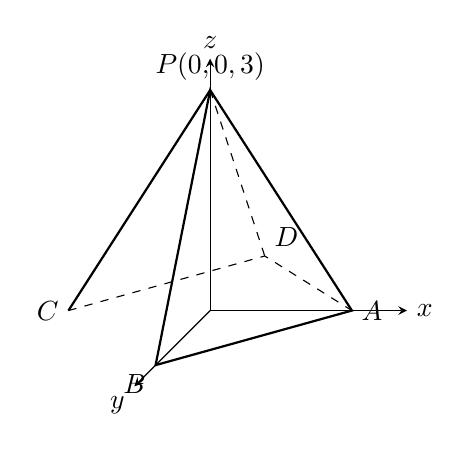
\begin{tikzpicture}[scale=1.0, >=stealth]
\draw[->] (0,0,0) -- (2.5,0,0) node[right] {$x$};
\draw[->] (0,0,0) -- (0,3.2,0) node[above] {$z$};
\draw[->] (0,0,0) -- (0,0,2.5) node[below left] {$y$};
\coordinate (P) at (0,2.8,0);
\coordinate (A) at (1.8,0,0);
\coordinate (B) at (0,0,1.8);
\coordinate (C) at (-1.8,0,0);
\coordinate (D) at (0,0,-1.8);
\draw[thick] (A) -- (B) -- (P) -- cycle;
\draw[thick] (P) -- (C);
\draw[dashed] (C) -- (D) -- (A);
\draw[dashed] (P) -- (D);
\node[above] at (P) {$P(0,0,3)$};
\node[right] at (A) {$A$};
\node[below left] at (B) {$B$};
\node[left] at (C) {$C$};
\node[above right] at (D) {$D$};
\end{tikzpicture}
\qquad
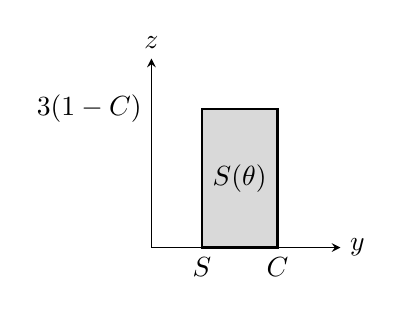
\begin{tikzpicture}[scale=0.8, >=stealth]
\draw[->] (0,0) -- (3,0) node[right] {$y$};
\draw[->] (0,0) -- (0,3) node[above] {$z$};
\draw[thick, fill=gray!30] (0.8, 0) rectangle (2.0, 2.2);
\node[left] at (0, 2.2) {$3(1-C)$};
\node[below] at (0.8, 0) {$S$};
\node[below] at (2.0, 0) {$C$};
\node at (1.4, 1.1) {$S(\theta)$};
\end{tikzpicture}
\end{center}

\bigskip

\noindent
\textbf{[解2]} 対称性から, $0 \le x \le 1$ での体積 $V'$ として,
\[
V = 4 V' \quad \dots \text{①}
\]
$x = C$ での切断面をかんがえる. $AP$ と $x^2 + y^2 = 1$ の交点が $E\left( \frac{1}{2}, \frac{1}{2}, \frac{3}{2}(2-\sqrt{2}) \right)$ であることに注意して, 右図をみる.
したがって,
\[
S(\theta) = \begin{cases} \frac{3}{2}(1-S)^2 & (\pi/4 \le \theta \le \pi/2) \\ \frac{3}{2}(1-C)^2 + 3(1-C)(C-S) & (0 \le \theta \le \pi/4) \end{cases}
\]
だから,
\begin{align*}
V' &= \int_0^1 S(\theta) \, dc = \int_{\pi/4}^{\pi/2} \frac{3}{2}(1-S)^2 S \, d\theta + \int_0^{\pi/4} \frac{3}{2}(1-C)^2 S \, d\theta + \int_0^{\pi/4} 3S(1-C)(C-S) \, d\theta \quad \dots \text{②}
\end{align*}
ここで,
\begin{align*}
\int_{\pi/4}^{\pi/2} (S^2 - 2S + 1) S \, d\theta &= 2 \left[ -C \right]_{\pi/4}^{\pi/2} + \frac{1}{3}[C^3]_{\pi/4}^{\pi/2} - \left[\theta - \frac{1}{2}\sin 2\theta\right]_{\pi/4}^{\pi/2} \\
&= \frac{11}{12}\sqrt{2} - \frac{1}{2} - \frac{\pi}{4} \\
\int_0^{\pi/4} (1-C)^2 S \, d\theta &= \left[ \frac{1}{3}(1-C)^3 \right]_0^{\pi/4} = \frac{5}{6} - \frac{7}{12}\sqrt{2} \\
\int_0^{\pi/4} 3S(1-C)(C-S) \, d\theta &= \frac{5}{12} + \frac{1}{2} - \frac{3}{8}\pi
\end{align*}
を②に代入して
\[
V' = \frac{3}{2}\left[\frac{11}{12}\sqrt{2} + \frac{5}{6} - \frac{\pi}{4}\right] + \frac{5}{12} + \frac{1}{2} - \frac{3}{8}\pi = (\sqrt{2}+1) - \frac{3}{4}\pi
\]
①から $V = 4(\sqrt{2}+1) - 3\pi$.

\end{document}
